\section{Problemstellung} \label{sec:Problemstellung}
Die fundamentale und schwerste Frage, bei den Stadt-Analogien ist, wie das Layout der Stadt aussehen soll. In Abschnitt \ref{sec:CodeCity} wurde das erste Layout vorgestellt, welches die Stadt-Analogie verfolgt. Die verbindende kompente dieser ARbeit ist, dass die 3D-Visualierung am Ende darüber entsteht, dass ein 2D-Layout generiert wird, welches dann durch eine weitere Metrik ins 3 dimensionale extrudiert wird. Und Anschließend weitere Metriken als einfärbung genutzt werden.


Die übergeordnete Frage dieser Arbeit, die sich aber gar nicht wirklich beantworten lässt, ist:

Welches Layout ist am besten geeignet, um Code-Qualitätsmetriken zu visualisieren? Gibt es bessere Layouts (als das von CodeCity), die eine bessere Übersichtlichkeit und Verständlichkeit bieten? 

Daraus leiten wir zwei konkrete Fragen ab, die in dieser Arbeit beantwortet werden sollen:
\begin{enumerate}
    \item Wie lassen sich die Treemap-Layout-Algorithmen für das konkrete Problem dieser Arbeit verbessern? Welche Vor- und Nachteile haben diese Anpassungen?
    \item Lassen sich über Recherche zu verwandten Arbeiten und bestehenden Tools Layouts finden, die sich besser eignen, um Code-Qualitätsmetriken zu visualisieren? 
    \begin{enumerate}
        \item Beispiel: Ist das Sunburst Layout besser geeignet als das "beste" Treemap-Layout, um Code-Qualitätsmetriken zu visualisieren?
        \item Beispiel: Ist das Stack Layout besser geeignet als das "beste" Treemap-Layout, um Code-Qualitätsmetriken zu visualisieren?
    \end{enumerate}
\end{enumerate}

Laut Marcus Adrian et al.  gibt es 5 Dimensionen die man beachten muss, wenn es um software visualierung geht: 
\begin{quote}    
    • Tasks - why is the visualization needed?
    • Audience - who will use the visualization?
    • Target - what is the data source to represent?
    • Representation - how to represent it?
    • Medium - where to represent the visualization? \cite[2]{3dsoftwareMarcus}
\end{quote}

Wir beantworten diese Fragen, um das Ziel dieser Arbeit zu begründen.
\textbf{Warum ist die Visualisierung von Codequalitätsmetriken wichtig?}
Die Visualisierung von Codequalitätsmetriken ist wichtig, um die Qualität von Softwareprojekten zu bewerten und zu verstehen, aber auch um einen schnellen Überblick über die Codebasis zu geben und einen Einstieg in vertiefende Codeanalysen zu ermöglichen. Eine effektive Visualisierung kann helfen, schnell Hotspots im Code zu identifizieren, die möglicherweise verbessert werden müssen, und somit die Wartbarkeit und Qualität des Codes zu erhöhen. Außerdem soll die Visualisierung ermöglichen verschiedene Metriken in verbindung zu setzen, um so eine höhere Aussagekraft über den Code, den die einzelne betrachtung jeder Metrik nicht bieten kann.
Der wichtigste Punkt ist, das subjektive \textit{Greifbar} machend der CodeQualität.

\textbf{Wer wird die Visualisierung nutzen?}
Die Visualisierung ist vorallem an Personen gerichtet, die sich nicht mit der Codebasis auskennen. Das können Entscheidungsträger sein, die keine ahung von software entwicklung haben, das können aber auch entwickler sein, die sich neu in ein Projekt einarbeiten müssen, um die qualität einer software zu erhöhen.

\textbf{Was ist die Datenquelle?}
Die Datenquelle sind hierarschiche Codequalitätsmetriken, die aus dem Quellcode eines Softwareprojekts extrahiert werden. 
Dabei wird jeder Knoten in dieser Hierarchie als "Node" bezeichnet.
Jede Node hat folgendes Schema:
```json
"node": {
    "name": string,
    "children": List[Node] | "value": number,
}
```


\textbf{Wo soll die Visualisierung dargestellt werden?}
Die Visualisierung soll digital auf herkömmlichen Bildschirmen dargestellt werden. Speziell wird in dieser Arbeit beispielhaft eine darstellung in einem Webbrowser angestrebt und die Algorithmen in Typescript implementiert. Natürlich können aber alle Ergebnisse auch in anderen Programmiersprachen und Umgebungen umgesetzt werden.


\textbf{Wie soll die Visualisierung dargestellt werden?}
Im GRunde soll eine Visualierung in Anlehnung an den in Abschnitt \ref{sec:CodeCity} beschriebenen Stadt-Metapher ansatz verfolgt werden. - Speziell soll es in dieser Arbeit um das Layout der Knoten gehen, aber im hinterkopf soll die stadtmetapher bleiben und immer als grundlage für die bewrtung des 2d layouts dienen. 
Wie in der CodeCity arbeit beschrieben, soll es möglich sein Metriken in form von Fläche, Höhe und farbe (ob jetzt nur farbe oder durchsichtigkeit wie bei dem codecity paper oder sogar textur von knoten - wird hier ignoriert). Das heißt also, dass das 2D layout in gewisser weise eingeschtränkt wird, zB. wenn Farbe als visulaisrung von struktur verwendet werden soll oder wie in \cite{bruls2000squarified} schattierung.

Speziell soll die Visualisierung am Ende optimiert auf folgende Aspekte sein, die sich aus den im Abschnitt \ref{sec:Grundlagen} beschriebenen Grundlegenden Aspekten von Softwarevisualierung, leicht angepasst and das Problem dieser Arbeit, ableiten lassen: 

\begin{itemize}
    \item \textbf{Informationsgehalt und Effiziente Nutzung des Platzes:} Die Visualisierung sollte so viele Informationen wie möglich auf so wenig Platz wie möglich darstellen.
    \item \textbf{Niedrige visuelle Komplexität und Verständlichkeit:} Als Gegenspieler zum Informationsgehalt steht die visuelle Komplexität. Die Visualisierung sollte so einfach und verständlich wie möglich gehalten werden, um den Betrachter nicht zu überfordern.
    \item \textbf{Skalierbarkeit:} Die Visualisierung sollte auch bei großen Software-Systemen noch gut lesbar sein. Dies ist besonders wichtig, da wir hier über große Software-Systeme sprechen.
    \item \textbf{Korrelation mit dem Code:} Die Visualisierung sollte eine gute Korrelation mit dem Code haben. Wenn man die Visualierung sieht, soll man diese auch mit dem Code in Verbindung bringen können. Es sollte also möglich sein, die Visualisierung mit dem Code zu verknüpfen und so ein besseres Verständnis für die Software zu bekommen.
    \item \textbf{Zweitrangig ist Stabilität gegenüber Änderungen:} Die Visualisierung sollte stabil gegenüber Änderungen in der Software sein, damit der Qualitätszustand der Software einfacher über die Zeit verfolgt werden kann.
\end{itemize}


\subsection{Das Treemap Problem} \label{sec:TreemapProblem}
In Abschnnit \ref{sec:Treemap} wurde aufgezeigt, dass bereits der initiale Algorithmus von Johnson und Shneiderman \cite{johnson1991tree} ein fundamentales Problem aufweist, wenn Treemaps mit Abständen zwischen Knoten dargestellt werden sollen. Zudem ist bereits das Problem, welches von Johnson und Shneiderman addressiert wird NP-Hard \cite[3]{bruls2000squarified} und das Problem mit Abständen macht es nicht einfacher.
\begin{itemize}
    \item Da der Abstand von der Fläche der Knoten abgezogen wird, ist die dargestellte Fläche nicht mehr proportional zum Wert des Knotens.
    \item Durch das Abziehen der Abstände kann es passieren, dass Knoten verschwinden, wenn entweder die Länge oder die Breite der Knoten kleiner oder gleich dem Abstand ist.
\end{itemize}

In den Abbildungen \ref{fig:zeroMarginArtificialMap}, \ref{fig:fiveMarginArtificialMap} und \ref{fig:tenMarginArtificialMap} sind Treemap Layouts abgebildet, die mit dem Squarify Algorithmus nach Abschnitt \ref{sec:Squarify} generiert wurden. Der Visualierten Metriken sind händisch erstellt, um das Problem zu verdeutlichen (siehe Anhang HIER REF EINRÜGEN). In Bild \ref{fig:zeroMarginArtificialMap} sind alle Knoten sichtbar und die Fläche der Knoten ist proportional zu den Werten der Knoten. In Bild \ref{fig:fiveMarginArtificialMap} sind immernoch alle Knoten sichtbar, aber die Fläche der Knoten ist nicht mehr proportional zu den Werten der Knoten. Zum Beispiel hat der Große Knoten mit Wert 3000 eine Fläche von ca. 2600, wärend der kleine Knoten oben links mit Wert 30 nur eine Fläche von ca. 5 hat. In Bild \ref{fig:tenMarginArtificialMap} mit Abstand 10 sind dann schon einige Knoten (zum beispiel der Eben genannte knoten oben links) nicht mehr sichtbar, da die breite der Knoten kleiner als der Abstand ist. 

\begin{figure}
    \centering
    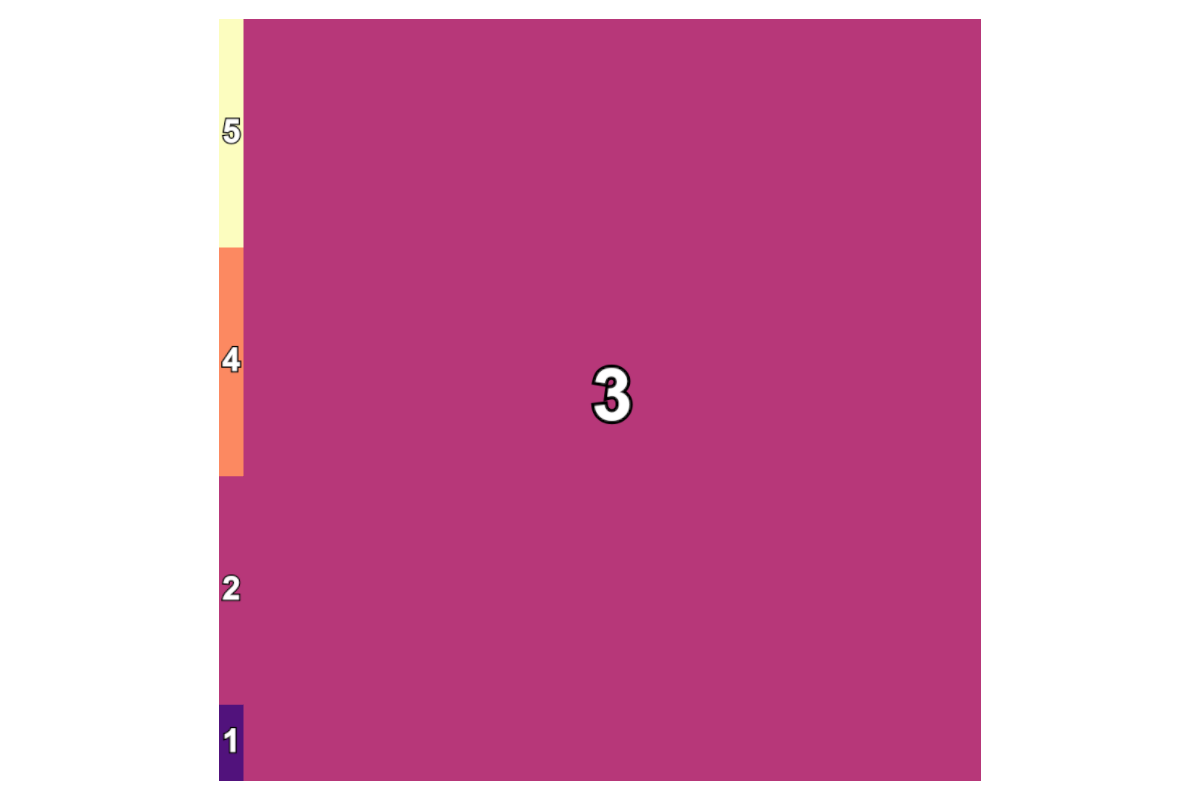
\includegraphics[width=0.8\textwidth]{images/zeroMarginArtificialMap.png}
    \caption{Treemap Layout generiert mit dem Squarify Algorithmus nach Abschnitt \ref{sec:Squarify} mit einem Abstand von 0} 
    \label{fig:zeroMarginArtificialMap}
\end{figure}

\begin{figure}
    \centering
    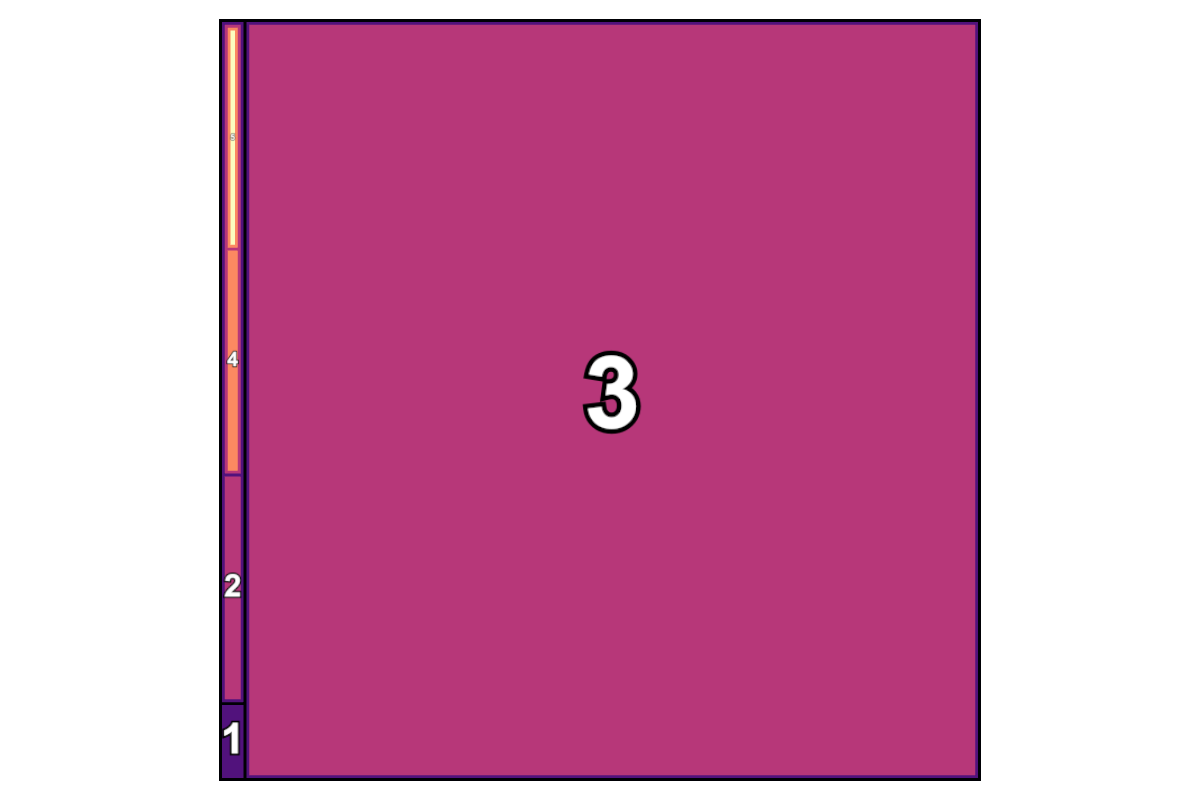
\includegraphics[width=0.8\textwidth]{images/fiveMarginArtifialMap.png}
    \caption{Treemap Layout generiert mit dem Squarify Algorithmus nach Abschnitt \ref{sec:Squarify} mit einem Abstand von 5} 
    \label{fig:fiveMarginArtificialMap}
\end{figure}

\begin{figure}
    \centering
    
\includegraphics[width=0.8\textwidth]{images/tenMarginArtifialMap.png}
    \caption{Treemap Layout generiert mit dem Squarify Algorithmus nach Abschnitt \ref{sec:Squarify} mit einem Abstand von 10} 
    \label{fig:tenMarginArtificialMap}
\end{figure}

Es ist nicht trivial dieses Problem zu lösen, da es die grundlegende Annahme der Treemap Algorithmen verletzt, dass die Fläche aller Knoten bekannt ist, bevor die Knoten plaziert werden. 
Bevor die Knoten plaziert werden, ist nicht klar, wie die Fläche der Knoten aussieht, das heißt, es ist auch nicht klar, wie viel Platz für die Abstände zwischen den Knoten benötigt wird. Dies wird klar wenn man sich die Abbildung \ref{fig:marginAreaDifference} anschaut. Dort sieht man, dass die Fläche, die für Knoten in ihren Eltern benötigt wird, größer ist als die Fläche, die für die Knoten selbst benötigt wird und diese benötigte Fläche stark vom Layout der Knoten selbst abhängt. Somit ist auch unklar, wie groß die Fläche aller elternknoten sind. 

\begin{figure}
    \centering
    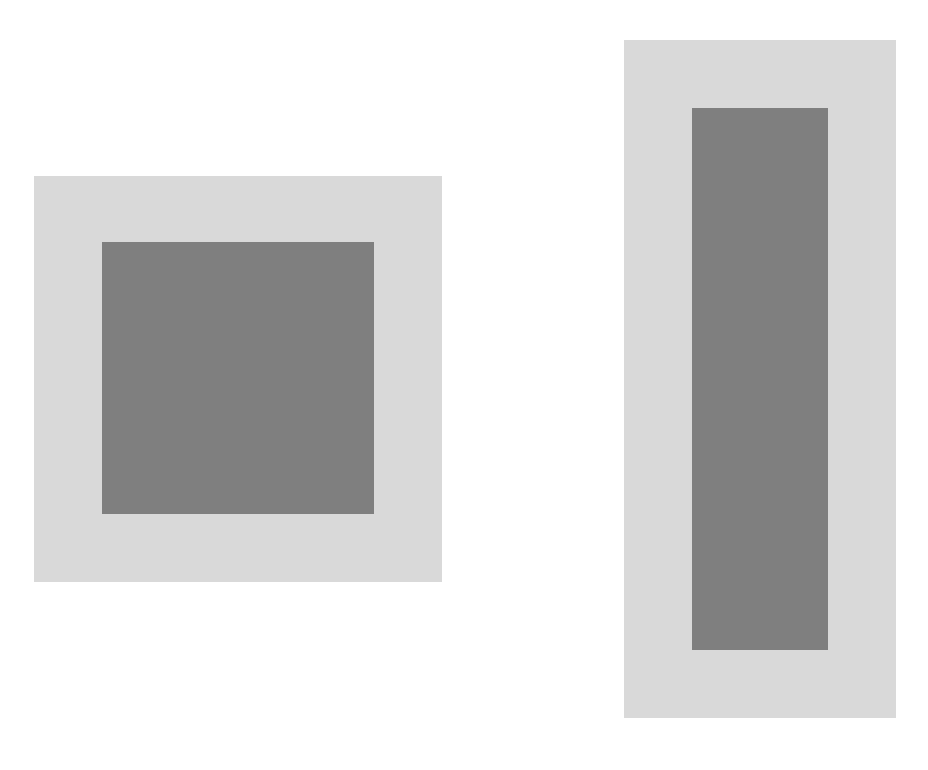
\includegraphics[width=0.8\textwidth]{images/marginArea.png}
    \caption{Abbildung eines zweier Rechecke mit der Fläche 16 in dunkel grau und in hellgrau der Abstand von 1 um die Flächen herum. Das Linke Rechteck (4x4) mit Abstand nimmt eine Fläche von 25 (5x5) ein. Das rechte Rechteck (2x8) mit Abstand nimmt eine Fläche von 40 (4x10) ein.}
    \label{fig:marginAreaDifference}
\end{figure}

Das Problem ist jetzt aber, dass wenn die Fläche der Knoten nicht bekannt ist auch das Layout der Knoten nicht berechnet werden kann, da die Fläche der Knoten für das Layout benötigt wird. Hier ergibt sich also ein Zirkelschluss: Die Fläche ist nicht klar, ohne das Layout und das Layout kann nicht berechnet werden, ohne die Fläche zu kennen.
